% !TEX root = morphkasten.tex

\section{Containererkennung (detailliert)}
Die Containererkennung muss auch ausgelegt sein für die Erkennung des Entladebehälters!

%##############
\subsection{Distanzsensor}
Die detaillierte Containererkennung mit Sensoren unterscheidet sich nur geringfügig von der groben Variante. Der Hauptunterschied besteht darin, dass bei der detaillierten Variante nur noch die Positionierung des Fahrzeugs vorzunehmen ist. Die Auswertung der Form und der Farbe wird Vorgängig von der Kamera erledigt und an das Mikrocontrollerboard weitergeleitet.
\begin{figure} [hbp]
	\centering
	\includegraphics[width=0.5\textwidth]{fig/Containererkennung_2.png}
	\caption{Beispielhafte Containererkennung mit Distanzsensoren (ohne Farbsensor)}
\end{figure}

\begin{table}[h]
\begin{tabular}{p{0.5\textwidth} | p{0.5\textwidth}}


 \textbf{Vorteile} & \textbf{Nachteile} \\ \hline
	 
\begin{itemize}
\item Präzise Erkennung des Containers (wahrscheinlich)
\item Mehrfachverwendung mit anderen Anwendungen denkbar
\item Kostengünstig (kein Farbsensor)
\end{itemize}

 
 &
 
\begin{itemize}
\item Unbekannte Präzision
\item Je nach Sensor Störanfälligkeit
\item Zusatzhardware und Verkabelung nötig
\end{itemize}

\end{tabular}
\end{table}

\begin{table}[h]
\begin{tabular}{p{0.5\textwidth}p{0.5\textwidth}}


 \textbf{Risiken} & \\ \hline
	 
\begin{itemize}
\item Die Sensoren sind zu ungenau
\item Die Sensoren werden gestört

\end{itemize}
&
\begin{itemize}
\item Die Kommunikation der groben und detaillierten Erkennung ist zu langsam
\end{itemize}

 
\end{tabular}
\end{table}

\pagebreak


%##############
\subsection{Bilderkennung}
\begin{figure}[h!]%Position festigen
\centering
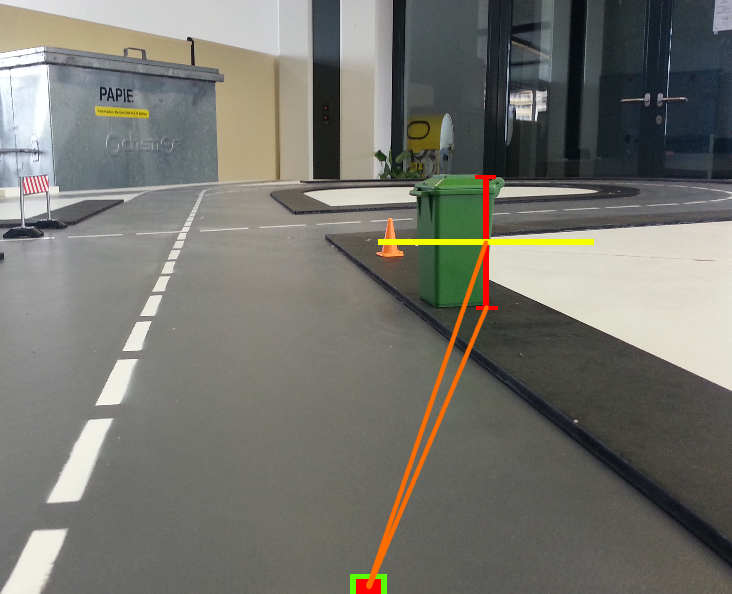
\includegraphics[width=0.7\textwidth]{fig/containererkennung_detailliert_bilderkennung.png}
\caption{Bilderkennung Container}
\label{fig:Bilderkennung Container}
\end{figure}
\begin{table}[h]
\begin{tabular}{p{0.5\textwidth} | p{0.5\textwidth}}


 \textbf{Vorteile} & \textbf{Nachteile} \\ \hline
	 
\begin{itemize}
\item Keine Sensoren zur Seite benötigt
\end{itemize}

 
 &
 
\begin{itemize}
\item Berechnung des Abstands muss auf wenige Milimeter stimmen
\item Keine Korrektur mehr möglich, wenn der Container aus dem Kamerbereich verschwindet oder zweite Kamera notwendig
\end{itemize}

\end{tabular}
\end{table}

\begin{table}[h]
\begin{tabular}{p{0.5\textwidth}p{0.5\textwidth}}


 \textbf{Risiken} & \\ \hline
	 
\begin{itemize}
\item Ungenauigkeit bei der Distanzabschätzung
\item Container kann zum Teil von anderen Gegeständen verdeckt sein
\end{itemize}

 
\end{tabular}
\end{table}

\pagebreak
